% coding:utf-8

\section{Digitally-Controlled Oscillator}

\subsection{Übersicht}
\begin{frame}
  \begin{center}
\tikzstyle{block} = [ draw,fill=blue!20,text width=5em,align=center,
                      rounded corners,minimum height=3em]
\def\radius{.7mm}
\tikzstyle{branch}=[fill,shape=circle,minimum size=3pt,inner sep=0pt]
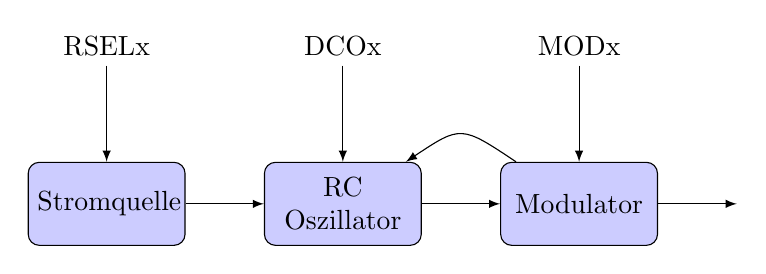
\begin{tikzpicture}
  \node[block] at (0,0) (iq) {Stromquelle};
  \node[block] at (3,0) (osc) {RC Oszillator};
  \node[block] at (6,0) (mod)   {Modulator};
  \node at (0,2) (rselx)   {RSELx};
  \node at (3,2) (dcox)   {DCOx};
  \node at (6,2) (modx)   {MODx};
  \draw[-latex] (iq.east) -- (osc.west);
  \draw[-latex] (osc.east) -- (mod.west);
  \draw[-latex] (mod.east) -- ++(right:1);
  \draw[-latex] (rselx.south) -- (iq.north);
  \draw[-latex] (dcox.south) -- (osc.north);
  \draw[-latex] (modx.south) -- (mod.north);
  \draw[-latex] (mod) .. controls (4.5,1) and (4.5,1) .. (osc);
%   \draw[-latex] (lfxt.east) -- (mclk.west);
%   \draw[-latex,dashed] (lfxt.east) -- (smclk.west);
%   \draw[-latex] (xt.east) -- (mclk.west);
%   \draw[-latex] (xt.east) -- (smclk.west);
%   \draw[-latex] (dco.east) -- (mclk.west);
%   \draw[-latex] (dco.east) -- (smclk.west);
\end{tikzpicture}
\end{center}

\end{frame}

% \begin{frame}
%     \frametitle{}
%     \framesubtitle{}
%       \begin{figure}
%         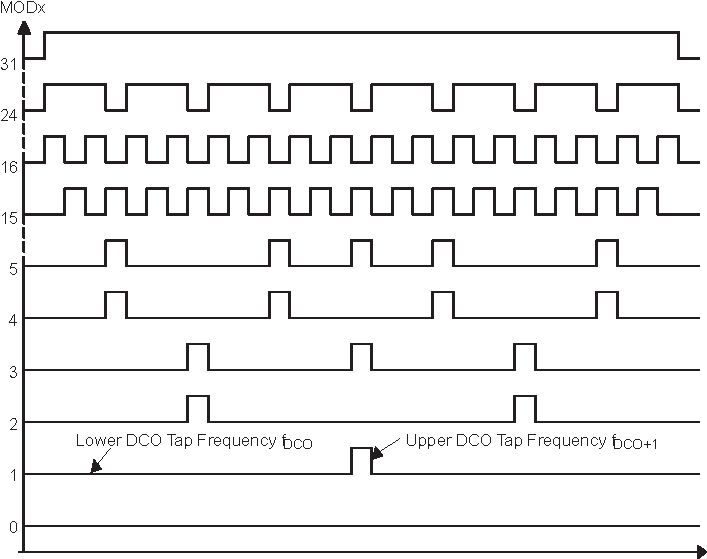
\includegraphics[width=0.7\columnwidth]{fig/ti_fg_dco_mod.pdf}
%         \caption{Funktionsweise Modulation}
%       \end{figure}
% \end{frame}

\subsection{Modulation}
\begin{frame}
  \begin{tikztimingtable}
    \mbox{\uncover<+->{MOD =  0}} & <.->33L<*>\\
    \mbox{\uncover<+->{MOD =  1}} & <.->16LH16L<*>\\
    \mbox{\uncover<+->{MOD =  2}} & <.->8LH15LH8L<*>\\
    \mbox{\uncover<+->{MOD =  3}} & <.->8L2{H7L}H8L<*>\\
    \mbox{\uncover<+->{MOD = 16}} & <.->L16{HL}<*>\\
    \mbox{\uncover<+->{MOD = 24}} & <.->L8{3HL}<*>\\
    \mbox{\uncover<+->{MOD = 31}} & <.->L31HL<*>\\
  \end{tikztimingtable}
\end{frame}